%Type of document
\documentclass[a4paper, 12pt]{report}

%For easy management of document margins and the document page size
\usepackage[right=3.5cm,left=3.5cm,top=3.5cm,bottom=3.5cm]{geometry}

%Allows to insert graphic files within a document
\usepackage{graphicx}

%Sup­ports com­pressed, sorted lists of nu­mer­i­cal ci­ta­tions, and also deals with var­i­ous punc­tu­a­tion and %other is­sues of rep­re­sen­ta­tion, in­clud­ing com­pre­hen­sive man­age­ment of break points
\usepackage{cite}

%It gives LaTeX the possibility to manage links within the document or to any URL when you compile in PDF
\usepackage{hyperref}

%To choose the font encoding of the output text
\usepackage[T1]{fontenc}

%To choose the encoding of the input text
%Consente di usare le lettere accentate
\usepackage[latin1]{inputenc}

%It provides the internationalization of LaTeX. It has to be loaded in any document, and you have to give %as an option the main language you are going to use in the document
\usepackage[english]{babel}
\usepackage{pdflscape}

%Provides compact, "starred" versions for the lists (itemize) 
\usepackage{mdwlist}

\normalfont
%Forza LaTeX ad una spaziatura uniforme, invece di lasciare più spazio
%alla fine dei punti fermi come da convenzione inglese
\frenchspacing
%Modifica della spaziatura interlineare
\linespread{1.3}

%Inizia il documento
\begin{document}

%Creazione di un frontespizio personalizzato
\begin{titlepage}

\begin{center}
\Large
\textbf{POLYTECHNIC UNIVERSITY OF MILAN} \\
\Large
School of Industrial and Information Engineering \\
Computer Science and Engineering
\end{center}

\addvspace{0.8cm}
%PER INSERIRE IMMAGINE
\begin{figure}[h]
\begin{center}

\includegraphics[width=3cm]{cpt/img/polimi}
\end{center}
\end{figure}

\addvspace{0.1cm}
\begin{center}
\LARGE

\textbf{Project of Software Engineering 2: MyTaxi Service \\
Project Plan}

\end{center}

\addvspace{0.5cm}
\Large
\begin{center}
\begin{tabular}{p{1\textwidth}p{0.3\textwidth}}
Course Professor: Prof. Elisabetta DI NITTO \\
\end{tabular}
\end{center}

\addvspace{0.6cm}
\Large
\begin{center}
\begin{tabular}{p{0.6\textwidth}p{0.6\textwidth}}
& Authors: \\
& Mattia 	CRIPPA		854126\\
& Francesca GALLUZZI	788328\\
& Marco 	LATTARULO	841399
\end{tabular}
\end{center}

\vfill
\Large
\begin{center}
Academic Year 2015--2016
\end{center}
\end{titlepage}

\clearpage

\tableofcontents
\clearpage

\chapter{Introduction}
\clearpage

\chapter{Function Points Approach} \label{chap2}
The Function Point approach is a technique that allows to evaluate the total dimension of the program and therefore the effort needed to develop the software product depending on its functionalities. 
The list of functionalities has been obtained from the RASD and from the Design Document. There are 5 types of Functional Points:

\begin{itemize}
	\item \textbf{Internal Logic File (ILF)}: a homogeneous set of data handled by the system.
	\item \textbf{External Interface File (ELF)}: a homogeneous set of data used by the application but handled by external application.
	\item \textbf{External Input}: elementary operation to elaborate data coming from the external environment.
	\item \textbf{External Output}: elementary operation that generates data for the external environment that usually includes also the elaboration of data from logic files
	\item \textbf{External Inquiry}: elementary operation that involves both input and output operations done without significant elaboration of data from logic files.
\end{itemize}
\clearpage

\begin{table}[!htbp]
\begin{center}
\begin{tabular}[t]{|p{0.3\textwidth}|c|c|c|}
\hline
\textbf{Function Types} & \textbf{Simple} & \textbf{Medium} & \textbf{Complex}\\
\hline
\hline
External Inputs & 3 & 4 & 6 \\
\hline
External Outputs & 4 & 5 & 7 \\
\hline
External Inquiries & 3 & 4 & 6 \\
\hline
Internal Logical Files & 7 & 10 & 15 \\
\hline
External Logical Files & 5 & 7 & 10 \\
\hline
\end{tabular}
\end{center}
\end{table}

\noindent Using the Function Points method and the table of weights above, we can calculate the FPs of the entire system as the sum of the FPs obtained by evaluating each one of the 5 types of Functional Points. In particular we are going to define a number of items for every type of FP and assign them a weight representing its complexity.

\begin{itemize}
	\item \textbf{Internal Logic File (ILF)}: The application includes a number of ILFs that will be used to store the information about \textit{passenger, taxi drivers, rides, routes and reservation / request calls}. Passenger and Taxi Driver entities have a simple structure as they are composed of a small number of fields; Ride and Route entities have a medium complex structure; Call entity instead has a complex structure. Thus, we can decide to adopt complex weight for Call, medium weight for Ride and Route and simple weight for Passenger and Taxi Driver entities. This means that we will come out with $2*7 + 1*10 + 1*15 = 49$ FPs concerning ILFs.
	\item \textbf{External Interface File (ELF)}: The application features only one EIF to manage the interaction with maps APIs. This information results in only one entity with a complex structure. Thus, we decide to adopt a complex weight. As a result, we get $1*10 = 10$ FPs.
	\item \textbf{External Input}: The application interacts with the user to allow him/her to:
	\begin{itemize}
		\item Login / Logout / Sign Up: these are simple operations, so we can adopt the simple weight for them: $3*3 = 9$ FPs.
		\item Reserve / Request a taxi: these are not a simple operation, so we can adopt the medium weight: $2*4 = 8$ FPs.
		\item Update Account: this is a simple operation so we can adopt a simple weight: $1*3 = 3$ FPs.
		\item Signal Availability: this is a simple operation so we can adopt a simple weight: $1*3 = 3$ FPs.
		\item Accept or Decline Call: this is a simple operation so we can adopt a simple weight: $1*3 = 3$ FPs.
		\item Insert Testing Code: this is a simple operation so we can adopt a simple weight: $1*3 = 3$ FPs.
	\end{itemize}
	As a result, we get $7*3 + 2*4 = 29$ FPs.
	\item \textbf{External Output}:
	\begin{itemize}
		\item After specific request, the application will provide information about incoming taxi to passengers: this operation is not too complex so we can adopt a medium weight: $1*5 = 5$ FPs.
		\item At the end of a ride, application will provide a receipt: this operation is not too complex so we can adopt a medium weight: $1*5 = 5$ FPs.
		\item The application delivers incoming requests to taxi drivers. This operation is simple so we can adopt a simple weight: $1*4 = 4$ FPs.
		\item The application provides to taxi drivers a certain amount of information about optimal routes and the ongoing ride. This operation is quite complex so we can adopt complex weight: $1*7 = 7$ FPs.
		\item The application allows taxi drivers to visualize the dashboard. This operation is not too complex so we can adopt medium weight: $1*5 = 5$ FPs.
	\end{itemize}
	As a result, we get $4 + 3*5 + 7 = 26$ FPs.
	\item \textbf{External Inquiry}: The application allows users to access some information. In particular user can see:
	\begin{itemize}
		\item Information about the system if he is a developer.
		\item The summary of receipts if he is a passenger.
		\item The summary of rides if he is a taxi driver.
	\end{itemize}
	Considering all these 3 operations as simple, we get $3*3 = 9$ FPs.
\end{itemize}

\noindent In summary, we have computed the following value for the unadjusted FPs: 123. This value can be used directly to estimate the effort in case we have some historical data that tell us how much time we usually take for developing a FP. Otherwise, it can be used as a basis to estimate the size of the project in SLOC and then use another approach such as COCOMO II to estimate the effort. \\
We use the standard conversion coefficient to compute the number of Source Lines Of Code (SLOC) starting from the FPs. Therefore:\\
$SLOC = 46 * FPs = 5658$ \\
where 46 is the value of the coefficient related to the specific framework we are using, Java EE, taken from the table at this web page: \href{http://www.qsm.com/resources/function-point-languages-table}{http://www.qsm.com/\\resources/function-point-languages-table}

\clearpage

\chapter{COCOMO II Approach} \label{chap3}
For carrying out this section of the document we are referring to the COCOMO II model definition manual at:\\
\href{http://csse.usc.edu/csse/research/COCOMOII/cocomo2000.0/CII\_modelman2000.0.pdf}{http://csse.usc.edu/csse/research/COCOMOII/cocomo2000.0/CII\_modelman\\2000.0.pdf}.\\
Following this document we have compiled the two tables below, and then we have used the online calculator at this web page: \href{http://csse.usc.edu/tools/COCOMOII.php}{http://csse.usc.edu/tools/\\COCOMOII.php} to compute the effort, the total cost, the duration and the number of person estimated for the completion of the project.

\begin{table}[!htbp]
\begin{center}
\begin{tabular}[t]{|p{0.3\textwidth}|p{0.15\textwidth}|c|}
\hline
\textbf{Scale Driver} & \textbf{Factor} & \textbf{Value} \\
\hline
\hline
Precedentedness & Very Low & 6,20 \\
\hline
Development Flexibility & Nominal & 3,04 \\
\hline
Risk Resolution & Low & 5,65 \\
\hline
Team Cohesion & Extra High & 0 \\
\hline
Process Maturity & High & 3,12 \\
\hline
\end{tabular}
\end{center}
\end{table}
\clearpage

\begin{table}[!htbp]
\begin{center}
\begin{tabular}[t]{|p{0.55\textwidth}|p{0.15\textwidth}|c|}
\hline
\textbf{Cost Driver} & \textbf{Factor} & \textbf{Value} \\
\hline
\hline
Required Software Reliability & Nominal & 1 \\
\hline
Data Base Size & Nominal & 1 \\
\hline
Product Complexity & Nominal & 1 \\
\hline
Required Reusability & High & 1,07 \\
\hline
Documentation match to life-cycle needs & High & 1 \\
\hline
Execution Time Constraint & Nominal & 1 \\
\hline
Main Storage Constraint & Nominal & 1 \\
\hline
Platform Volatility & Nominal & 1 \\
\hline
Analyst Capability & Low & 1,19 \\
\hline
Programmer Capability & Nominal & 1 \\
\hline
Application Experience & Low & 1,10 \\
\hline
Platform Experience & Low & 1,09 \\
\hline
Language and Tool Experience & Nominal & 1 \\
\hline
Personnel Continuity & Very Low & 1,29 \\
\hline
Usage of Software Tools & Nominal & 1 \\
\hline
Multisite development & Low & 0,86 \\
\hline
Required Development Schedule & Nominal & 1 \\
\hline
\end{tabular}
\end{center}
\end{table}

\begin{figure}[!htbp]
\centering
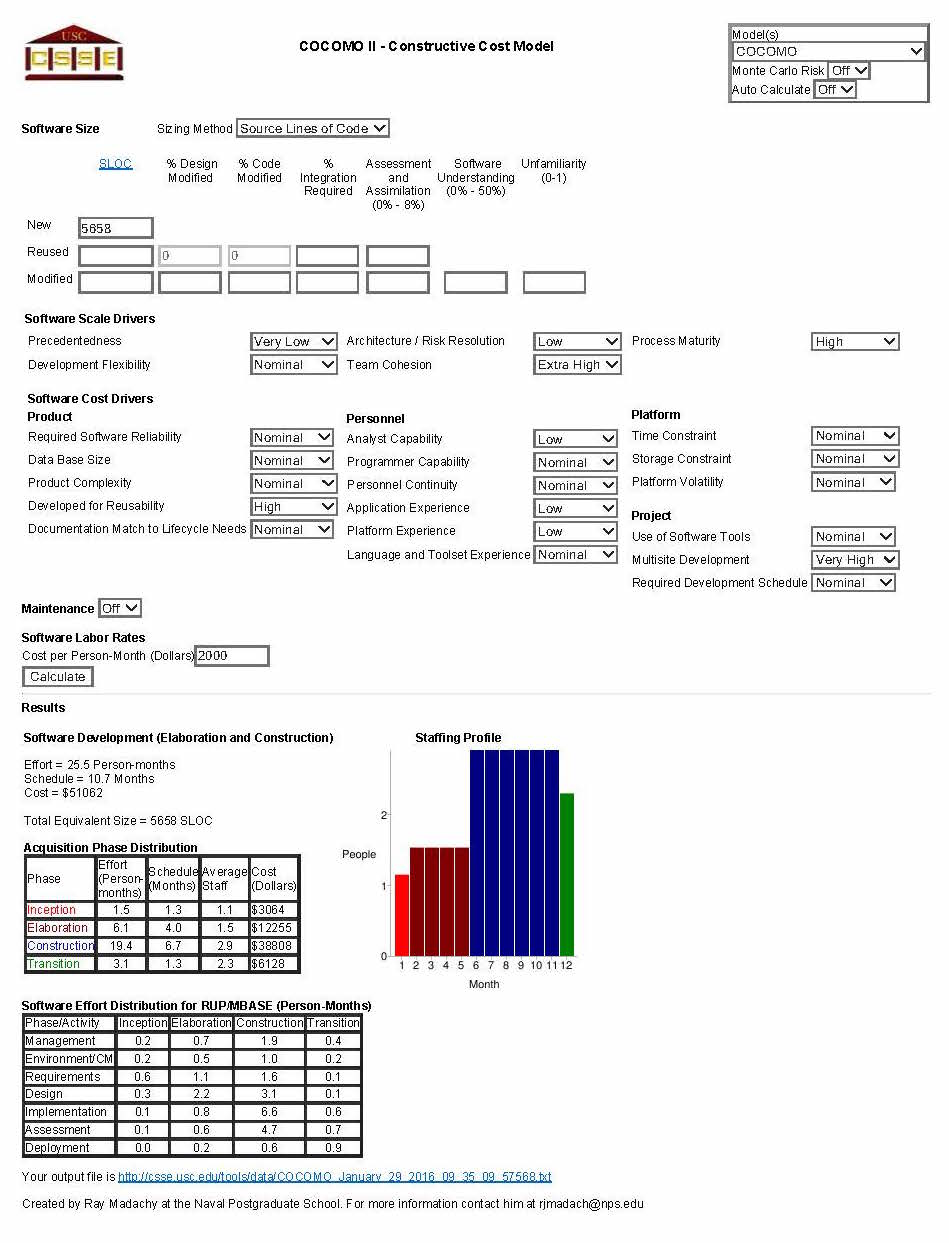
\includegraphics[width=\textwidth]{cpt/img/COCOMOII-ConstructiveCostModel}
\caption{Representation of effort, total cost, duration and number of person estimated for the completion of the project.}
\end{figure}

\noindent So, in conclusion we have found these values for effort, total cost, duration and members of the project:\\
\textbf{Effort} = 25,5 Person-Months \\
\textbf{Cost} (assuming an average cost per Person-Month of 2.000,00 \$) = 51.062,00 \$ \\
\textbf{Duration} = 10,7 months \\
\textbf{Team size} = $25,5 / 10,7 = 2,38$ members \\
\clearpage

\chapter{Project Schedule \& Resources Allocation} \label{chap4}
In defining the possible schedule for the project we have tried to adhere as much as possible to the result of the previous evaluation made using FP and COCOMO II adapting those prescriptions to our specific case (a team composed of 3 people).
We have identified 6 major tasks to carry out during the development of the project:
\begin{itemize}
	\item T1 : Feasibility study
	\item T2 : Analysis of Requirements and specifications
	\item T3 : Design of the system
	\item T4 : Coding and Unit testing
	\begin{itemize}
		\item T4.1 : Client Side
		\item T4.2 : Server Side
		\item T4.3 : Database
	\end{itemize}
	\item T5 : Integration test and system test
	\item T6 : Deployment
\end{itemize}
In the effort of balancing as much as possible the workload of each component of the team we have developed the following Gantt diagram (Figura \ref{fig:scheduele}) showing the distribution of every task among the team members during the months, forecasting a total duration of 10 months (rounding down with respect to the prescription obtained using COCOMO II to balance the dimension of the team - 3 people instead of 2,38).

\begin{figure}[!htbp]
\centering
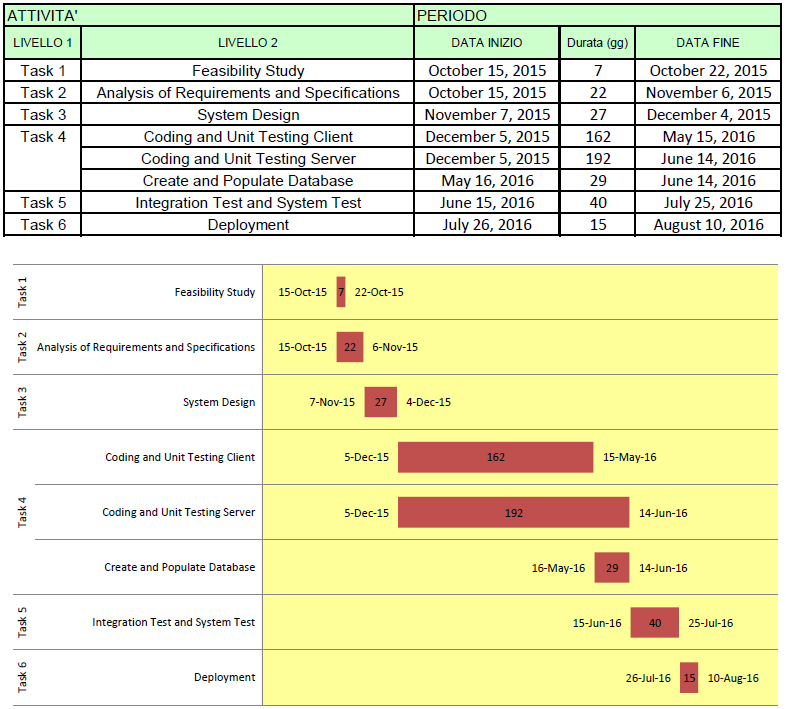
\includegraphics[width=\textwidth]{cpt/img/Schedule}
\caption{Project schedule}
\label{fig:scheduele}
\end{figure}
\clearpage

\noindent In Figure \ref{fig:staffalloc} instead is represented how the staff will be allocated in order to accomplish each task.

\begin{figure}[!htbp]
\centering
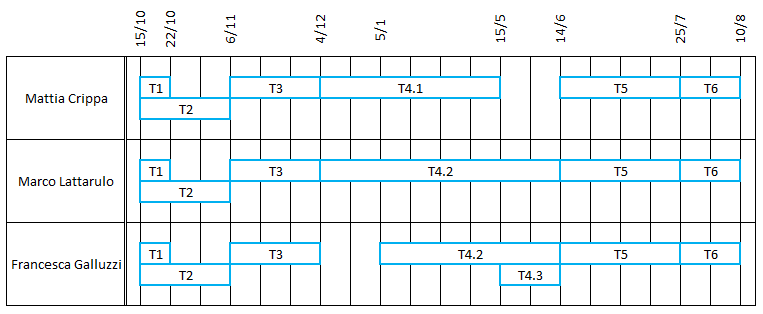
\includegraphics[width=\textwidth]{cpt/img/StaffAlloc}
\caption{Staff Allocation Chart}
\label{fig:staffalloc}
\end{figure}
\clearpage

\chapter{Project Risks} \label{chap5}
Given the nature of the project and the small dimension of the group of developers (3 person), the major risks are related to the availability of all the members of the team and to the respect of the time schedules. In fact, every member of the team has the same importance and has more or less the same skills of the other, so it's not possible to fully replace one team member in a short time, and it's also difficult for the two remaining members to carry out the scheduled tasks efficiently, in case of illness or unavailability of the third member.
Also from the small number of developers depend all the possible risks related to unexpected modifications to the design of the system or also to the scheduling. The lack of hierarchy and the uniformity of skills lead to a necessity of continuous meetings and sharing of ideas and works. All this leads to small reactivity to changes and longer development time.
One possible idea for solving or preventing such problems is to enlarge the team or at least to involve other people in some of the aspect of the project, and try to make all the documentation as much complete and effective as possible, so to make easier and faster for a new member the ingress in the team and the understanding of what's going on.
Another possible idea is to better organize the distribution of the tasks in the team, trying to reach an optimal balance between collaboration and individual work. Trying to enforce collaboration only on the fundamental tasks and enforce decoupling on all the other minor tasks.

\clearpage

\chapter{Other Information} \label{chap6}

\section{Working Hours}

\begin{table}[htbp]
\begin{center}
\begin{tabular}[t]{ccc}

\hline
\textbf{First Name} & \textbf{Last Name} & \textbf{Total Hours} \\
\hline
Mattia & Crippa &  16h\\
\hline
Francesca & Galluzzi &  16h\\
\hline
Marco & Lattarulo & 17h\\
\hline

\end{tabular}
\end{center}
\end{table}
\clearpage

\end{document}
